\documentclass{template/sig-alternate-05-2015}

\usepackage{natbib}
\usepackage[brazil]{babel}
\usepackage{multicol}
\usepackage{multirow}
\usepackage{hyperref} % Required for hyperlinks


\hypersetup{hidelinks,colorlinks,breaklinks=true,urlcolor=color2,citecolor=color1,linkcolor=color1,bookmarksopen=false,pdftitle={Title},pdfauthor={Author}}

\makeatletter

\def\portkeywords#1{\g@addto@macro\@keywords{\endgraf\bigskip{\bfseries\Large\noindent
      PALAVRAS-CHAVE}\endgraf\noindent#1}}%

\newenvironment{otherlangabstract}{\Collect@Body\@saveaotherbstract}{}

\long\def\@saveaotherbstract#1{\g@addto@macro\@abstract{\endgraf\bigskip{\bfseries\Large\noindent
      RESUMO}\endgraf\noindent\ignorespaces#1}}

\@saveaotherbstract{}

\makeatother

\begin{document}
\setcopyright{acmcopyright}

\title{Análise de Características a partir de Algoritmos de
  Aprendizagem de Máquina para Auxílio ao Diagnóstico do Transtorno do
  Espectro Autista}

\numberofauthors{1} \author{
  \alignauthor Matheus Frota, Samuel
  Hericles, Gerônimo Aguiar, Pedro Renoir, Rayon Nunes, Manoel Vilela,
  Denilson Gomes, Iális Cavalcante
  \\
  \affaddr{Universidade Federal do Ceará - Campus de Sobral}\\
  \affaddr{Engenharia da Computação, Sobral-CE, Brasil}\\
  \email{ \texttt{matheusfrota@hotmail.com.br},
    \texttt{samuel.herilces@alu.ufc.br}, \texttt{geron@alu.ufc.br},
    \texttt{renoir@alu.ufc.br}, \texttt{rayonnunes@hotmail.com},
    \texttt{manoel$\_$vilela@engineer.com},
    \texttt{denilsongomes@alu.ufc.br}, \texttt{ialis@sobral.ufc.br} }
}

\maketitle
\begin{abstract}

  % Abstract.
  Machine learning algorithms are being successfully applied in many
areas of knowledge. In digital health, these ones permit for
professionals to be helped to diagnose diseases and disorders in
advance and more accurately, contributing to the effective treatment
of their patients. In this context, the proposed methodology makes use
of a public database on Autistic Spectrum Disorder and the most
relevant characteristics presented by a patient. So, it analyzes with
the Decision Tree, Support Vector Machine, Multi-Layer Perceptron and
K-nearest neighbor algorithms to the construction of a model capable
of simplifying a decision strategy to help the diagnosis of this
disorder type.\\
  \textbf{keywords:}{Autism, Machine learning, Feature importance.}\\

\end{abstract}

\begin{otherlangabstract}
  \textbf{Resumo}.
  Algoritmos de aprendizado de máquina estão sendo
aplicados com sucesso em diversas áreas do conhecimento. No campo da
saúde, estes mesmos abrem espaço para que profissionais possam ser
auxiliados a diagnosticar doenças e transtornos antecipadamente e com
maior precisão, contribuindo no tratamento eficaz de seus
pacientes. Neste contexto, a metodologia proposta faz uso de uma base
de dados pública sobre o Transtorno do Espectro Autista e as
características mais relevantes apresentada por um paciente. Para
isso, analisa com os algoritmos de Árvore de Decisão, \textit{Support
Vector Machine}, Perceptron de Múltiplas Camadas e K-vizinhos mais
próximos a construção de um modelo capaz de simplificar uma estratégia
de decisão no auxílio ao diagnóstico deste tipo de transtorno.\\
  \textbf{palavras-chaves:}{Autismo, Aprendizagem de máquina,
    Importância de características.}
\end{otherlangabstract}

\newpage

\section{Introdução}

Desde maio de 2013 os psicólogos e psiquiatras estão utilizando os
critérios de avaliação do Manual de Diagnóstico e Estatístico de
Transtorno Mentais (conhecido como DSM-5), elaborado pela
\textit{American Psychiatric Association} \cite{autismspeaks}. Os
casos anteriormente analisados, utilizando o DSM-IV, que recebiam o
diagnóstico de transtorno autista, transtorno de \emph{Aspeger} ou
transtorno de desenvolvimento penetrante, que não seja especificado de
outra forma, passam a ser nomeados de transtorno do espectro autista,
podendo ainda ser caracterizado em 3 (três) diferentes níveis de
gravidade. Os sintomas desses transtornos representam um contínuo
único de prejuízos às pessoas portadoras, com intensidades variáveis,
que vão de leve a grave, nos domínios de comunicação social e de
comportamentos restritivos e repetitivos. Este estudo destaca que o
transtorno do espectro do autismo (TEA), refere-se a uma ampla gama de
condições caracterizadas por desafios com habilidades sociais,
comportamentos repetitivos, fala e comunicação não-verbal
\cite{APA2014}.

O autismo afeta cerca de 1 em 59 crianças hoje nos Estados
Unidos. Dessa forma, estima-se que o Brasil, com seus 200 milhões de
habitantes, possua cerca de 3 milhões de autistas. O autista possui um
conjunto distinto de traços comportamentais. As maneiras pelas quais
as pessoas com autismo aprendem, pensam e resolvem problemas podem
variar de muito qualificadas a severamente desafiadas pela situação
\cite{de2019analise}.

Tendo em vista a problemática de alcançar o diagnóstico do autismo, o
presente trabalho propõe um método para auxiliar especialistas na
busca por um diagnóstico deste transtorno. Com base em dados público
sobre um grupo crianças autistas, pretende-se analisar características
descritas na base de dados junto as informações necessárias cedidas
pelos responsáveis, acelerando o procedimento. Para colaborar com a
análise de muitos dados, adota-se alguns algoritmos relevante na
literatura sobre aprendizagem de máquina para buscar uma análise
automática de auxílio aos especialistas
\cite{Talabani:2018,Thabtah:2018,Yuan:2012}. Foram utilizados quatro
tipos de algoritmos, visando a classificação das características
comportamentais em crianças, com um determinado grau de autismo ou
não. É importante destacar a ideia principal, que visa apenas fornecer
um auxílio com a previsão ao diagnóstico. Caso o resultado seja
positivo significa que a criança pode apresentar algum grau de autismo
e, portanto, o especialista pode fazer uso dos resultados desta
aplicação como base para o laudo final.

O artigo está organizado como segue. Na seção 2 descreve-se os
trabalhos relacionados à classificação e TEA. Na seção 3 é descrita
toda estrutura da base de dados utilizada, apontando os atributos
utilizados. A seção 4 aborda toda a fundamentação teórica do
trabalho. Na seção 5 são apresentados os resultados obtidos, mostrando
o gráfico de importância das variáveis utilizadas no modelo. Por fim,
a seção 6 conclui o trabalho e sugere aplicações futuras.

\section{Trabalho relacionados}

Teixeira \textit{et al.} (2010) realiza uma revisão sistemática, nos
anos de 2002 a 2009, a cerca da produção científica de autores
brasileiros relacionados ao TEA. A pesquisa foi realizada partir das
bases de dados públicas em 4 (quatro) diferentes repositórios,
incluindo diversos descritores, tais como autismo e transtorno
invasivo do desenvolvimento. Houve a análise de 93 artigos, em que
aproximadamente um terço dos mesmo foi publicado em periódicos, mas a
maioria dos artigos se baseava em amostras pequenas. Notou-se que o
principal tema de pesquisa abordado estava ligado a programas de
intervenção para TEA. Ao final, a referida revisão dispôs sobre o
interesse de pesquisadores brasileiros na temática dos TEA,
entretanto, a maior parte dessa produção científica se concentra em
dissertações/teses em detrimento de poucas publicações em revistas
relevantes. Esta revisão sistemática mostrava que há muito tempo
faz-se necessário a abertura de novos estudos com amostras maiores que
levariam a um maior impacto e visibilidade da produção científica
brasileira relativa aos TEA \cite{TEIXEIRA:2010}.

Em Brito \& Fernandes (2019) foi proposto o uso de redes neurais para
classificar crianças com presença ou não de TEA. Utilizaram uma base
de dados com 259 amostras e com as estratégias de \textit{cross
  validation} e \textit{k-fold} para auxílio no treinamento. Os dois
modelos comportaram-se bem mas os autores deram como inconclusivo os
seus resultados \cite{de2019analise}.

Processamento de imagens e algoritmos de aprendizado de máquina foram
empregados por Liu \textit{et al.} (2016) para classificar crianças
com autismo. Os dados foram de rosto de crianças junto com um conjunto
de dados do movimento ocular dessas, por fim obtiveram um acurácia de
88,51$\%$ nos resultados \cite{Wenbo}.

A proposta de Halibas \textit{et al.} (2018) analisa cinco modelos de
aprendizado de máquina para estudar o problema da desordem do espectro
autista em uma base específica. Os autores fazem um comparativo entre
os modelos com as métricas de acurácia, precisão e revocação. A base
de dados utilizada foi definida a partir de 1100 amostras com 10
atributos comportamentais, sendo crianças, adolescentes e adultos. As
amostras já possuem a classe conhecida: "Pertencente" ou "Não
Pertencente" ao espectro autista. Este estudo apontou o classificador
baseado em \textit{Deep Learning} como o modelo que alcança melhor
desempenho em quase todas as métricas, com acurácia de 96,38\%
\cite{Halibas:2018}.

O trabalho de Dutta \textit{et al.} (2017) mostra um modelo de
aprendizagem de máquina como método para auxiliar o diagnóstico do
autismo em crianças, mas também mostra sua aplicação na previsão de
outras síndromes e transtornos, mas tendo seu melhor funcionamento
para a previsão do autismo. Sua proposta envolve uma Regra de
Associação (AR) baseado em um método de valor mínimo de Redundância e
Máxima Relevância (mRMR), usados para extrair os sintomas que precisam
ser testados para o processo de previsão, a partir de uma base de
dados. Foi utilizado o método de Diferença de Informação Mútua (MID)
junto ao maior ganho de informação (HIG) para selecionar os sintomas
adicionais, através de casos anteriores, e que podem estar vinculados
aos sintomas principais \cite{Dutta:2017}. O método de diagnóstico
recebe informações de vários sensores e smartphones. Os dados do
sensor são buscados através de um aplicativo por um aparelho
mobile. Executando o aplicativo, os sintomas preliminares tentam puxar
os sintomas associados em várias iterações do banco de dados através
da Internet.  O banco de dados utilizado contém registros de pacientes
anteriores com sintomas padrão. O tal sistema proposto precisa de um
ou dois sintomas primários como entradas para seu funcionamento, os
sintomas são ainda testados e confirmados. O procedimento foi feito em
um conjunto de 200 crianças portadoras de transtornos variados, com 10
tipos de autismos e 50 sintomas distintos. Os resultados obtidos na
aplicação de tal método para todos os casos envolveram taxas entre 70
a 86\% de precisão. No geral, os experimentos demonstraram
funcionamento bem melhor para casos específicos, mais voltados ao
desenvolvimento intelectual das crianças, onde pode ainda se ter uma
melhor recuperação no desenvolvimento cognitivo. Ao mesmo tempo, não
se mostra tão eficiente para casos que demonstram uma maior
dificuldade na socialização da criança, por exemplo. Por fim, o artigo
faz ressalvas sobre os exames de sintomas preliminares que geralmente
não são suficientes para uma boa previsão do início do autismo em
crianças, e que sintomas preliminares acabam indicando diferentes
diagnósticos \cite{Dutta:2017}.

Este transtorno também foi avaliado em algoritmos de aprendizagem de
máquina não supervisionados. Em Elbattah \textit{et al.} (2019), a
idéia principal é aprender agrupamentos de dados com base na
representação visual de percursos de rastreamento ocular. Levando em
consideração que o TEA é uma condição ao longo da vida caracterizada
por prejuízos sociais e de comunicação, analisou o rastreamento ocular
de 59 crianças organizadas em dois grupos: autistas e
não-autistas. Aplicou-se a tecnologia de eye-tracking para
rastreamento das variações de direcionamento das visões dos pacientes
que se deparavam com imagens de formas e geravam caminhos de visadas
entre os mesmos. Avaliou-se três hipóteses principais: Os padrões
visuais dos caminhos de rastreamento de rastreamento ocular indicariam
uma estrutura subjacente de grupos?  Se sim, os aglomerados
descobertos poderiam revelar possíveis conexões relacionadas à
dinâmica do comportamento do olhar (por exemplo, velocidade,
aceleração)? Além disso, como os agrupamentos variariam em relação às
características dos participantes (por exemplo, idade)? O modelo de
agrupamento foi treinado usando representações compactadas aprendidas
por um autoencoder profundo \cite{Albuquerque:2018}. Seus resultados
atingiram uma tendência promissora da estrutura de agrupamento. Além
disso, os grupos são explorados para fornecer informações
interessantes sobre as características do comportamento do olhar
envolvido no autismo. Confirmou-se empiricamente que os caminhos de
rastreamento ocular podiam ser agrupados em grupos coerentes, que se
assemelhavam amplamente ao agrupamento original de amostras (ou seja,
autistas ou não-autistas). Isso traz um significado nas visualizações
do caminho de digitalização que podem efetivamente discriminar as
amostras diagnosticadas com autistas e outros grupos
\cite{Elbattah:2019}.

No artigo de Sartipi, Shayesteh \& Kalbkhani (2018) faz-se uso de
algoritmos de aprendizado de máquina em aplicações médicas a fim de
permitir um diagnóstico rápido e preciso de doenças, em específico
para o caso de TEA. Seu objetivo é classificar entre autistas e
não-autistas usando as informações de dados de ressonância magnética
funcional incluindo os de em estado de repouso (do inglês
\textit{Resting State functional Magnetic Resonance Imaging},
rs-fMRI). Em sua proposta, cada região de interesse (do inglês
\textit{Region of Interest}, ROI) de dados de cada sujeito é
decomposta usando a transformada wavelet discreta
\textit{double-density dual-tree} (D3TDWT) dem sub-bandas de
frequência de tempo. Num momento seguinte, o modelo de
heteroscedasticidade condicional auto-regressiva generalizada (do
inglês \textit{generalized autoregressive conditional
  heteroskedasticity}, GARCH) é usado para a extração de recursos
dessas sub-bandas. Posteriormente, as características mais
discriminantes são selecionadas pelo teste-t de duas amostras e,
finalmente, os dados são classificados por \textit{Support Vector
  Machine}. Este foi testado em vários conjuntos de dados e os
resultados atingiram uma precisão de classificação de 71,6\% para
indivíduos do sexo masculino e, para o sexo feminino,
93,7\%. Considerando os ROIs significativos, há uma redução nas
conexões ântero-posteriores entre os autistas, e que pode ser
considerado em abordagens clínicas \cite{Sartipi:2018}.

A metodologia apresentada em Akter \textit{et al.} (2019) destaca que
(TEA) é um grupo de deficiências no desenvolvimento neurológico que
não são curáveis, mas que podem ser amenizado por intervenções
precoces. O referido trabalho abordou um conjuntos de dados de
autistas detectados precocemente em grupos de bebês, crianças,
adolescentes e adultos e aplicou vários métodos de transformação de
recursos. Várias técnicas de classificação foram implementadas com
esses conjuntos de dados, que foram transformados e avaliados em seu
desempenho. Notou-se que o SVM mostrou o melhor desempenho para o
conjunto de dados da criança, enquanto que o GLMboost para os
adolescentes, e o Adaboost apresentou os melhores resultados para o
conjunto de dados da criança e de adultos. As transformações de
recursos que resultam na melhores classificações foram função seno
para a criança e \textit{z-score} para conjuntos de dados de crianças
e adolescentes. Após estas análises, várias técnicas de seleção de
recursos foram usadas com esses conjuntos de dados transformados em
\textit{z-score} para identificar os fatores de risco significativos
de TEA nos grupos de diferentes faixas etárias. Os resultados destas
abordagens analíticas indicam que, quando adequadamente otimizados, os
métodos de aprendizado de máquina podem fornecer boas previsões de
estado de autismo. Isso sugere que pode ser possível aplicar esses
modelos para a detecção de autismo em seus estágios iniciais
\cite{Akter:2019}.

Algumas estratégias de uso de algoritmos de aprendizagem de máquina
foram centradas em comitê de classificadores. O mesmo pode-se tratas
do trabalhar de Yuan \& Ma (2012), que já destacava que as tentativas
existentes de melhorar o desempenho do AdaBoost em conjuntos de dados
desequilibrados têm se concentrado amplamente na modificação de sua
regra de atualização de peso ou na incorporação de amostras ou
técnicas de aprendizado sensíveis a custos. Os autores buscaram
modelar um comitê de classificadores com uma nova
perspectiva. Inicialmente, o conjunto de dados passa por uma
superamostragem e o AdaBoost padrão é aplicado para criar uma série de
classificadores básicos. Em seguida, os pesos dos classificadores são
novamente treinados por algoritmos genéticos ou técnicas de otimização
comparáveis, nas quais medidas de desempenho mais direcionadas podem
ser usadas diretamente como função objetivo. Consequentemente, essa
estratégia de amostragem unida à reponderação pode propositalmente
ajustar o AdaBoost em direção a uma determinada medida de desempenho
de interesse. Resultados experimentais em dez conjuntos de dados de
benchmark mostram que essa estratégia pode aumentar o desempenho do
AdaBoost de maneira confiável e tem superioridade consistente sobre
outros métodos associados e que são apresentados na literatura
\cite{Yuan:2012}.

O trabalho de Gok (2019) também destaca que o diagnóstico de TEA nos
estágios iniciais é muito desejável para estabelecer o tratamento
rapidamente. Do ponto de vista do aprendizado de máquina, a tarefa de
previsão de risco de autismo é uma classificação binária dos genes de
risco de autismo, ou seja, se um RNA longo não codificado (do inglês
\textit{long non-coding RNA}, lncRNA) causa o transtorno ou
não. Buscou-se desenvolver um modelo de aprendizado de máquina,
treinado a partir de dados de expressão gênica no desenvolvimento
cerebral, para a classificação binária dos genes de risco de
autismo. O modelo foi composto de duas partes principais: extração de
recursos com transformada de wavelet de Haar, métodos de discretização
e classificação com o algoritmo de aprendizado de rede
bayesiana. Apresentou-se uma comparação o modelo proposto em outros
algoritmos de classificação independentes que abordaram dados sobre o
gene lncRNA. Os resultados experimentais obtiveram uma importante
eficiência do modelo, principalmente com a sensibilidade, área sob
curva ROC e pontuações da medida F1-Score de 90,2\%, 83,9\%,e 80,6\%,
respectivamente \cite{Gok:2019}.

O estudo de Usta \textit{et al.} (2019) segue uma linha de pesquisa
junto a outros trabalhos que mostram melhorias parciais em alguns
sintomas principais dos TEA com o decorrer do tempo. No entanto, os
fatores preditivos (por exemplo, pré-tratamento, distúrbios
psiquiátricos comórbidos, habilidades adaptativas e de linguagem etc.)
para melhorar o resultado não foram estudados com métodos de
aprendizado de máquina. O objetivo dos autores envolveu examinar os
cálculos preditores de resultados com métodos de aprendizado de
máquina, incluindo estimativa estatística, teorias da informação e
aprendizado matemático, descobrindo automaticamente padrões úteis em
grandes quantidades de dados. Adotou-se um grupo de amostras que
compreendeu 433 crianças (na faixa de 3 a 6 anos de idade) com
diagnóstico de TEA. Os sintomas das mesmas foram avaliados pela Lista
de Verificação do Comportamento do Autismo, Lista de Verificação do
Comportamento Aberrante e escalas de Impressão Clínica Global (do
inglês \textit{Clinical Global Impression}, CGI)\cite{Usta:2019}. Foi
avaliado o desempenho de algoritmos de aprendizado de máquina (Naive
Bayes, Modelo Linear Generalizado, Regressão Logística, Árvore de
Decisão) nos referidos dados, incluindo os 254 itens nos formulários
de linha de base. Pacientes com menos de 2 pontos de CGI nos sintomas
de TEA em 36 meses foram aceitos como o grupo que apresentou de melhor
resultado para a classe de previsão. Uma proporção significativa dos
casos apresentou melhora significativa nos sintomas de TEA. No modelo
de aprendizado de máquina assumido em uma escala CGI mostrou-se que o
grupo de diagnóstico afetou o prognóstico. No grupo de autismo, pai e
mãe mais velhos, menor peso ao nascer e maior idade no diagnóstico
apresentam pior resultado. Na idade do transtorno de Asperger no
diagnóstico, a idade da primeira avaliação e os pilares do
desenvolvimento afetaram o prognóstico. Acompanhando outros trabalhos
na literatura, identificou-se diagnóstico precoce, reabilitação
precoce e severidade dos sintomas de TEA na avaliação inicial do
resultado previsto. Além disso, observou-se que diagnósticos
psiquiátricos comórbidos estão afetando o resultado dos sintomas de
TEA na observação clínica. Os modelos de aprendizado de máquina
revelam que vários outros são mais significativos (por exemplo, idade
dos pais, peso ao nascer, variáveis sociodemográficas, etc.) em termos
de informações prognósticas e também no planejamento do tratamento de
crianças com TEA \cite{Usta:2019}.

A pesquisa de Abbas \textit{et al.} (2018) engloba dois algoritmos
treinados para identificar o autismo. Um destes é baseado em
questionários estruturados e curtos, relatados pelos pais. E o outro
algoritmo usa a identificação de comportamentos-chave a partir de
vídeos caseiros semiestruturados de crianças. Um algoritmo de
combinação é então usado para combinar os resultados em uma única
avaliação de maior precisão. Para superar a escassez e desequilíbrio
dos dados de treinamento, aplicou-se técnicas de seleção de
características, \textit{feature engineering} e técnicas de
codificação de características. Permitiu-se uma determinação
inconclusiva, quando apropriado, a fim de aumentar a precisão da
triagem quando conclusiva. O desempenho é então validado em um estudo
clínico controlado, que se seguiu com 162 crianças para verificar o
desempenho desses algoritmos e sua combinação. Atingiu-se uma melhoria
significativa da precisão em relação às ferramentas de triagem padrão
nas medições de acurácia, sensibilidade e especificidade. O estudo
assegura que um processo de aprendizado de máquina é um método
confiável para a detecção de autismo fora dos ambientes clínicos. Uma
variedade de fatores de confusão na análise clínica é discutida
juntamente com as soluções projetadas nos algoritmos. Os resultados
finais são estatisticamente limitados e demandam futuros estudos
clínicos para ampliar o tamanho da amostra \cite{Abbas:2018}.

A abordagem de Ben-Sasson, Robins \& Yom-Tov (2018) possui o objetivo
de testar a viabilidade da avaliação do risco de desordem do espectro
do autismo nas preocupações dos pais a partir de fontes baseadas na
Web, usando ferramentas de análise de texto automatizadas e
questionamento de padrão mínimo. Os participantes desta pesquisa eram
115 pais, preocupados com o desenvolvimento da comunicação social de
seus filhos. As crianças tinham entre 16 e 30 meses de idade e 66 das
mesmas tinham histórico familiar de transtorno do espectro do
autismo. Os pais relataram suas preocupações na internet e completaram
um questionário para um rastreador específico em TEA, a Lista de
Verificação Modificada e Revisada para Autismo em Crianças (do inglês
\textit{Modified Checklist for Autism in Toddlers-Revised}). Fizeram
uso também de um amplo rastreador de desenvolvimento, denominado
Questionário de Idades e Estágios (do inglês \textit{Ages and Stages
  Questionnaire}, ASQ). Um algoritmo previa o risco de distúrbio do
espectro do autismo usando uma combinação do texto dos pais e uma
única pergunta de triagem, selecionada pelo algoritmo para aprimorar a
precisão da previsão. As medidas de triagem identificaram 58 a 88\%
das crianças em risco de desordem do espectro autista. Crianças com
histórico familiar de TEA apresentaram três vezes mais chances de
apresentar risco de transtorno do espectro do autismo nas medidas de
triagem. A previsão do risco de uma criança no ASQ ou na lista de
verificação foi significativamente mais precisa quando prevista a
partir do texto combinado com uma pergunta selecionada automaticamente
do que apenas no texto. As perguntas da lista de verificação
frequentemente selecionadas automaticamente que previam risco eram:
seguir um ponto, brincadeira de faz de conta e preocupação com
surdez. Observou-se que a internet pode ser usada para pré-rastrear
distúrbios do espectro do autismo, usando as preocupações dos pais,
administrando algumas perguntas de triagem padronizadas para aumentar
esse processo \cite{Sasson:2018}.

Com essa revisão dos trabalhos relacionados foi possível entender a
problemática de análise de crianças e outros grupos etários com
características de TAE, além da complexidade de se aplicar técnicas de
aprendizagem de máquina nesse âmbito das bases de dados
disponíveis. Este trabalho assume uma análise das características que
mais caracterizam o TAE em um paciente sobre o resultado de um
algoritmo de classificação de dados.

\section{Base de dados}

A base de dados utilizada neste trabalho, disponível em
\cite{Thabtah2017}, conta com um total de 292 observações e 21
atributos. Dentre esses atributos, tem 10 variáveis comportamentais
que são descritas na Tabela \ref{tab:confusao1}.

\begin{table}[!h]

        \begin{tabular}{|c|l|}
          \hline
          \textbf{Variável} & \multicolumn{1}{c|}{\textbf{Descrição}}                                            \\ \hline
          A1\_Score         & Alta percepção em baixos ruídos que && geralmente outros não percebem              \\ \hline
          A2\_Score         & Maior concentração na visão do todo em && comparação a pequenos detalhes           \\ \hline
          A3\_Score         & Facilidade de comunicação com várias pessoas && diferentes ao mesmo tempo          \\ \hline
          A4\_Score         & Facilidade de fazer múltiplas tarefas && simultaneamente                           \\ \hline
          A5\_Score         & Dificuldade de manter uma conversa com && seus colegas                              \\ \hline
          A6\_Score         & Facilidade em manter conversas informais                                           \\ \hline
          A7\_Score         & Dificuldade de percepção de intenções e && sentimentos em histórias                 \\ \hline
          A8\_Score         & Dificuldade de brincar com a imaginação && fugindo da realidade                     \\ \hline
          A9\_Score         & Facilidade de reconhecer sentimentos && a partir de expressões faciais alheias     \\ \hline
          A10\_Score        & Dificuldade de fazer novas amizades                                                 \\ \hline
          result            & Soma das características comportamentais && avaliadas relacionados ao TEA.         \\ \hline
          Class/ASD         & Decisão do algoritmo sobre a criança && pertencer ou não ao espectro autista       \\ \hline
        \end{tabular}

        \caption{Variáveis comportamentais}
        \label{tab:confusao1}
      \end{table}

      \section{Fundamentação Teórica}

      Nesta seção são destacados os principais métodos que foram
      utilizados para a caracterização das variáveis em
      estudo. Destacam-se aqui o método de classificação de Árvore de
      Decisão, K-Vizinhos Mais Próximos (do inglês \textit{K-Nearest
        Neighbors} - KNN), Perceptron de Múltiplas Camadas, Support
      Vector Machine (SVM) e a função de avaliação (\textit{Feature
        Importance}).


      \subsection{Árvore de Decisão}

      O algoritmo de Árvore de Decisão se mostrou uma técnica bem
      adequada para o trabalho por apresentar na base de dados
      variáveis assumidamente binárias. Esta técnica pode ser definida
      como uma estrutura de dados que determina uma classe como um nó
      folha, um nó decisão que contém algum teste sobre um atributo e,
      a cada resultado, uma aresta para uma subárvore
      \cite{Rezende1999}.

      Este algoritmo tem algumas vantagens, como reduzir a
      complexidade do problema em regiões de decisão. É possível
      aproximar espaços de alta-dimensionalidade em vários níveis da
      árvore e conjunto de dados com muitas
      características. Permite-se ainda estimar um agrupamento menor
      desses em cada nó da árvore para testar com outros subconjuntos
      para melhorar a performance do algoritmo. Porém, com grandes
      bases de dados,os erros podem se acumular ao longo dos níveis da
      árvore de decisão e não podendo otimizar precisão e eficiência
      ao mesmo tempo \cite{IEEE}.

      \subsection{K-Vizinhos Mais Próximos}

      O algoritmo dos vizinhos mais próximos é um dos modelos
      preditivos mais simples e com diversas aplicações
      \cite{Dutta:2017,joel,Halibas:2018}. Cada amostra de uma base de
      dados $D$ é considerada a partir de um vetor $X$ com $l$
      dimensões, onde $X = [x_{1}, x_{2}, ...,x_{l}] \in R^{l}$. A saída
      é determinada de acordo com o parâmetro $K$, ou seja, o rótulo
      de maior incidência nos $k$ vizinhos mais próximos. Em caso de
      empate existem várias técnicas, mas as mais usadas são escolhas
      aleatórias do vencedor, ou reduzir o valor de $K$ até achar um
      vencedor absoluto.


      \subsection{Perceptron de Múltiplas Camadas}

      Um modelo de rede neural bastante aplicado na literatura é o
      Perceptron de Múltiplas Camadas, do inglês \textit{Multi-Layer
        Perceptron} (MLP)
      \cite{Hyde:2019,Thabtah:2018,zaji2019application}. Resume-se
      esse algoritmo de redes neurais como uma das várias técnicas
      inspiradas em um neurônio biológico, sendo este representado
      matematicamente por uma unidade que recebe dados de entrada
      $x_i$ e somadas junto com pesos $w_i$ que dão mais importância a
      certos valores de entradas do que outros. Após este efeito,
      realiza-se a soma de todos esses valores e subtrai-se do total
      um valor que filtra o contingente comum a todos, que é
      denominado \textit{bias} $\Theta$. Segue-se com o cálculo do
      resultado $u$ que é passado por uma função de ativação $g(u)$
      que, dependendo do resultado, ativa ou não a saída do neurônio
      \cite{HAYKIN:2001}, conforme pode-se visualizar na Figura
      \ref{fig:mlp1}.

    \begin{figure}[!h]
      \centering
      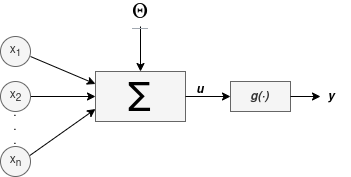
\includegraphics[width=.4\textwidth]{imagens/neuronio.png}
      \caption{Estrutura matemática de um neurônio em redes neurais.}
      \label{fig:mlp1}
    \end{figure}

    Dessa maneira, uma rede MLP utiliza as unidades matemáticas dos
    neurônios em determinadas camadas: a camada de entrada em que os
    padrões são apresentados à rede; a oculta onde é feita a maior
    parte do processamento através das conexões ponderadas, e que
    podem ser consideradas para extração de características; e a
    camada de saída onde o resultado final é concluído e apresentado
    \cite{zaji2019application}.

    \subsection{Support Vector Machine}

    Outro algoritmo de treinamento para aprendizado de máquina
    abordado é o Support Vector Machine (SVM). Este é utilizado para
    reconhecimento de padrões baseado na Teoria de Aprendizagem
    Estatística \cite{samsudin2010hybrid}, utilizado comumente para
    classificação, mas também é possível utilizá-lo para
    regressão. Objetos de entradas são vistos como pontos pertencentes
    ao hiperplano $R^l$, em que $l$ é a quantidade de atributos. O SVM
    traça um plano separador entre esses pontos dividindo-os em duas
    classes. Um problema é dito linearmente separável se for possível
    separar as classes usando um plano de dimensão $l-1$. Isso pode
    ser facilmente estendido à classificação de $k$ classes
    construindo $k$ classificadores de duas classes cada. A
    interpretação geométrica do SVM traz uma busca da separação ideal
    de uma superfície. Ou seja, formar o hiperplano que seja
    equidistante das duas classes em questão \cite{Talabani:2018}.

    \subsection{Feature Importance}

    A medida \textit{Feature Importance} trata-se do processo de busca
    das melhores variáveis que descrevem um determinado modelo. A
    Equação \ref{eq1} destaca o comportamento dessa medida, com base
    nas técnicas de \textit{impureza de Gini}, ou \textit{redução
      média das impurezas}, que calcula a importância de cada
    característica de entrada no resultado do modelo
    \cite{IEEE}. Desse modo, seu valor é calculado pela soma das
    frequências das classes sobre o número total delas.

    \begin{equation}
      \textit{G} = \sum_{j=1}^J P_j(1 - P_j)\label{eq1}
    \end{equation}

    Destaca-se na Equação \ref{eq1} que $G$ varia de (0,1] e
    representa o grau de importância da variável $j$ no modelo, $J$ é
    a quantidade de classes e $P$ representa a frequência de uma
    categoria.

    Para o cado específico da Árvore de Decisão, deve-se atentar ao
    cálculo de $\hat{\Gamma}(t)$. As classes são divididas em nós que são
    características para classificar as amostras do conjunto de
    dados. Assim, seja $\hat{\phi_j}(t)$ a frequência de uma classe
    $j$ em um nó $t$, a impureza de Gini \cite{Mach} aplicada ao nó
    $t$ é definida na Equação \ref{eq2}. Logo, cada nó é avaliado a
    partir dessa métrica.

    \begin{equation}
      \hat{\Gamma}(t) = \sum_{j=1}^J \hat{\phi_j}(t)(1-\hat{\phi_j}(t))
      \label{eq2}
    \end{equation}

    \subsection{Matriz de Confusão}

    A matriz de confusão permite analisar de forma detalhada o
    comportamento de um classificador, e para isso ela divide os
    resultados em quatro tipos \cite{Talabani:2018}:

    \begin{itemize}
    \item \textbf{Verdadeiro Positivo (VP)}: Se refere aos casos que o
      modelo previu corretamente a classe positiva.
    \item \textbf{Verdadeiro Negativo (VN)}: Se refere aos casos que o
      modelo previu corretamente a classe negativa.
    \item \textbf{Falso Positivo (FP)}: Se refere aos casos onde o
      modelo previu que era de uma classe positiva mas na verdade era
      da classe negativa.
    \item \textbf{Falso Negativo (FN)}: Se refere aos casos onde o
      modelo previu que era de uma classe negativa mas na verdade era
      da classe positiva.
    \end{itemize}

    A matriz de confusão em um problema binário, como o que está sendo
    abordado na base em questão (autista ou não-autista), pode ser
    configurado de acordo com a Tabela \ref{tab:mc}.

    \begin{table}
      \caption{Exemplo de Matriz de Confusão}\label{tab:mc}
      \centering
      \begin{tabular}{cccc}
        &
        & \multicolumn{2}{c}{Valor Previsto} \\ \cline{3-4}
        & \multicolumn{1}{c|}{}
        & \multicolumn{1}{c|}{Positivo}
        & \multicolumn{1}{c|}{Negativo}        \\ \cline{2-4}
        \multicolumn{1}{c|}{\multirow{2}{*}{\begin{tabular}[c]{@{}c@{}}Valor\\ Real\end{tabular}}}
        & \multicolumn{1}{c|}{Positivo} & \multicolumn{1}{c|}{\begin{tabular}[c]{@{}c@{}}Verdadeiros\\ Positivos\end{tabular}}
        & \multicolumn{1}{c|}{\begin{tabular}[c]{@{}c@{}}Falsos\\ Negativos\end{tabular}}
        \\ \cline{2-4} \multicolumn{1}{c|}{}
        & \multicolumn{1}{c|}{Negativo} & \multicolumn{1}{c|}{\begin{tabular}[c]{@{}c@{}}Falsos\\ Positivos\end{tabular}}
        & \multicolumn{1}{c|}{\begin{tabular}[c]{@{}c@{}}Verdadeiros\\ Negativos\end{tabular}} \\ \cline{2-4}
      \end{tabular}
      \label{tab:my_label}
    \end{table}

    \subsection{Métricas de Desempenho}
    \label{sec:mt}

    A partir da matriz de confusão é possível utilizar métricas que
    podem ser assumidas para analisar o desempenho do
    classificador. Dentre estas métricas, tem-se a \textit{Accuracy},
    que define qual a porcentagem de acertos do classificador. Outra
    medida é a \textit{Precision} que identifica quantos casos
    classificados como corretos estavam realmente corretos. Há ainda a
    \textit{Recall}, que avalia com que frequência o classificador
    aborda os exemplos de uma classe. E por último, destaca-se a
    \textit{F1-Score} (F1) que combina Precisão e Revocação em uma
    média harmônica e indica a qualidade geral do modelo. As
    definições matemáticas de \textit{Accuracy}, \textit{Precision},
    \textit{Recall} e \textit{F1-Score} estão dispostas nas Equações
    \ref{eqA} a \ref{eqF1}, respectivamente.

    \begin{equation}
      Accuracy = \frac{VP + FP}{VP+VN+FP+FN}
      \label{eqA}
    \end{equation}

    \begin{equation}
      Precision = \frac{VP}{VP+FP}
      \label{eqP}
    \end{equation}

    \begin{equation}
      Recall = \frac{VP}{VP+FN}
      \label{eqR}
    \end{equation}

    \begin{equation}
      F1 = \frac{2*Recall * Precision}{Recall+Precision}
      \label{eqF1}
    \end{equation}

    \section{Resultados e testes}

    Ao aplicar os classificadores destacados à base de dados, foi
    possível observar a taxa de erros, a performance de cada um e
    extrair as características mais influentes na decisão do modelo. O
    trabalho avalia ao final qual a melhor classificação e análise dos
    dados contidos na base mencionada.

    \subsection{Matriz de Correlação}

    Para a construção de um modelo consistente, faz-se necessário a
    seleção de variáveis descorrelacionadas entre si. Destaca-se que
    dadas duas variáveis análogas, há uma redundância de informações
    que poderá afetar o desempenho do modelo. Dessa forma, para
    analisar a correspondência entre as variáveis, desenvolveu-se a
    matriz de correlação como visto na Figura~\ref{fig:correlacao}.

    \begin{figure}[!h]
      \centering
      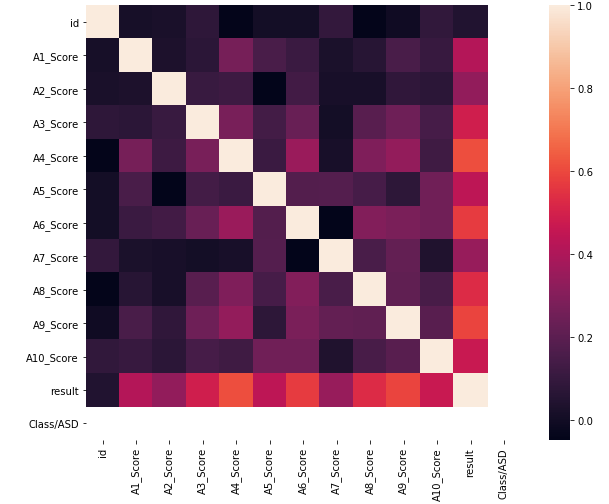
\includegraphics[width=.5\textwidth]{imagens/correlacao.png}
      \caption{Matriz de Correlação}
      \label{fig:correlacao}
    \end{figure}

    Em seguida, pode-se observar uma correlação de no máximo que 0,35
    em um índice no intervalo absoluto [0, 1] das variáveis de entrada
    entre si. E ainda, um índice mais alto na correlação entre as
    variáveis de entrada e a variável resposta. Isso indica que as
    variáveis de entrada não são correlacionadas entre si, e possuem
    correlação relevante com a variável resposta.

    \subsection{Avaliação das características}\label{sec:5.2}

    Os gráficos dessa seção apresentam a classificação das
    importâncias das variáveis de acordo com o algoritmo de
    aprendizado de máquina. Em cada um dos mesmos é mostrado também um
    \textit{boxplot} por característica, em que se definem os valores
    máximo, mínimo, \textit{outliers}, mediana e medidas de tendências
    de dispersão.


    No modelo de vizinhos mais próximos (\emph{k-NN}), o primeiro
    parâmetro configurado é $k$ que representa o número de vizinhos a
    serem considerados, valor este que apresentou melhor desempenho
    foi o valor 1 (um). A análise das características mais relevantes
    com esse modelo está disposto na Figura \ref{fig:knn}. Destacam-se
    as características A1, A9, A4, A10 e A7 com importância maior que
    $0,04$. As duas primeiras características, apesar de apresentarem
    alguns \textit{outliers}, dispõe de maior relevância dentre as
    demais de acordo com suas variabilidades. A4 possui valores
    superiores a A10 e A7 (estas praticamente empatadas) mas com alta
    variabilidade em suas ocorrências.

    \begin{figure}[!h]
      \centering
      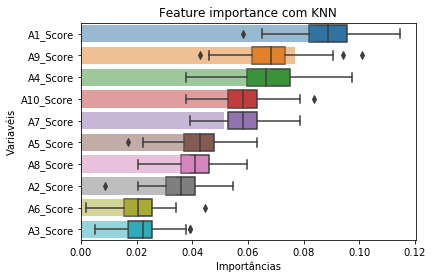
\includegraphics[width=.5\textwidth]{imagens/box_knn.png}
      \caption{Importância das variáveis no modelo KNN}
      \label{fig:knn}
    \end{figure}

    No modelo de rede neural \emph{MLP} foi utilizado apenas uma
    camada oculta com $20$ neurônios e $150$ iterações. Além disso,
    aplicou-se o otimizador de pesos Broyden-Fletcher-Goldfarb-Shanno
    (BFGS) que é um método baseado em derivadas que realiza as
    atualizações usando as informações do gradiente do modelo
    \cite{Maciel:2016}. Por fim, definimos em $0,1$ o valor do termo
    de regularização ou penalidade dos pesos para prevenir
    \textit{overfitting}, penalizando pesos com grandes valores. O
    gráfico sobre a importância das características pode ser
    visualizado na Figura \ref{fig:mlp}. Evidenciam-se variabilidades
    quase que em mesma escala para a maioria das características, mas
    informações das medianas de A1, A10 e A4, com importância maior
    que $0,08$ apesar da presença de \textit{outliers}.

    \begin{figure}[!h]
      \centering
      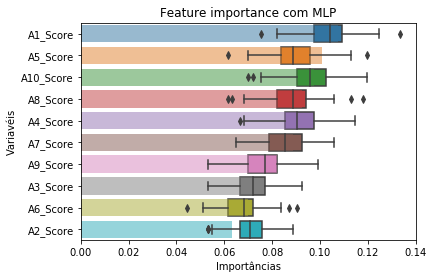
\includegraphics[width=.5\textwidth]{imagens/box_mlp.png}
      \caption{Importância das variáveis no modelo MLP}
      \label{fig:mlp}
    \end{figure}

    Com o modelo SVM foi adotado \textit{kernel} linear que atua como
    o produto interno das entradas com uma função não linear
    \cite{samsudin2010hybrid}. A análise das características mais
    relevantes com esse modelo está disposto na Figura
    \ref{fig:svm}. Destacam-se as características A1, A10, A4 e A7 com
    importância maior que $0,09$. Mesmo que as duas primeiras
    características apresentem alguns \textit{outliers}, estas se
    destacam com maior relevância dentre as demais de acordo com suas
    variabilidades. Para esse modelo, todas as variáveis obtiveram
    relevência com mediana acima de $0,06$.

    \begin{figure}[!h]
      \centering
      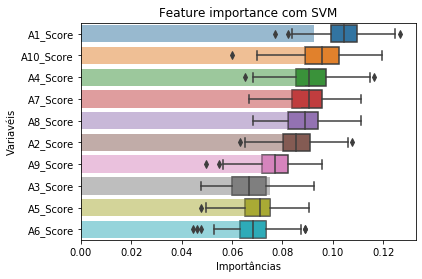
\includegraphics[width=.5\textwidth]{imagens/box_svm.png}
      \caption{Importância das variáveis no modelo SVM}
      \label{fig:svm}
    \end{figure}

    Para o método de AD assumiu-se alguns parâmetros nos
    experimentos. Primeiramente definiu-se um valor inteiro igual a
    100 (cem) que representa justamente a profundidade máxima da
    árvore em questão. O segundo parâmetro envolve a estratégia usada
    para escolher a divisão em cada nó, que foi assumida como
    aleatória. Por fim, aplicou-se um valor inteiro igual a 2 (dois)
    para o número mínimo de amostras necessárias em um nó
    folha. Assim, um ponto de divisão em qualquer profundidade terá
    esse valor mínimo em cada um dos ramos. A Figura \ref{fig:ad} é
    exibida com a análise das características mais relevantes para a
    Árvore de Decisão. As características A4, A10, A9, A3, A1 e A7 com
    importância maior que $0,05$. As duas primeiras características
    apresentam maior relevância dentre as demais de acordo com suas
    variabilidades.

    \begin{figure}[!h]
      \centering
      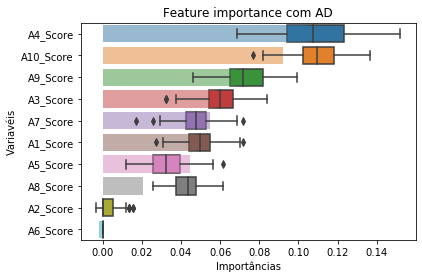
\includegraphics[width=.5\textwidth]{imagens/box_ad.png}
      \caption{Importância das variáveis no modelo de árvore de
        decisão}
      \label{fig:ad}
    \end{figure}

    Levando em consideração as Figuras \ref{fig:knn} a \ref{fig:ad},
    percebe-se que as variáveis A1, A10 e A4 alcançaram maior destaque
    na maioria dos experimentos apresentados nos quatro modelos. Os
    algoritmos \emph{SVM} e \emph{MLP} expressaram um perfil mais
    parecido entre eles no comportamento das importâncias dentre as
    características. Todas com um grau de importância maior que nos
    demais métodos, em termos gerais. As variáveis nos modelos
    \emph{KNN} e \emph{AD} que trouxeram maior variância de relevância
    entre as mesmas. As diferenças entre as importâncias das
    características tiveram comportamento mais similar que entre as
    demais abordagens. Estes dois últimos métodos possuem menor
    demanda de aproximação dos dados em decorrência dos ajustes de
    seus parâmetros.

    \subsection{Curva de Aprendizagem}

    A Curva de Aprendizagem é um gráfico que dispõe o desempenho do
    modelo de Aprendizagem de Máquina ao longo dos ciclos de
    experimentos. A partir dos gráficos produzidos é possível
    diagnosticar problemas com o aprendizado, além de identificar se
    os dados de treinamento e validação são adequadamente
    representativos \cite{joel,HAYKIN:2001,zhang2019overfitting}.

    Na Figura \ref{fig:feature1} pode-se acompanhar o comportamento da
    curva de aprendizagem do modelo de Árvore de Decisão. Nota-se que
    quando o tamanho da base de dados de treino aumenta o desempenho
    nos dados de treino e de teste vai convergindo em um ponto de alto
    desempenho.

    \begin{figure}[!h]
      \centering
      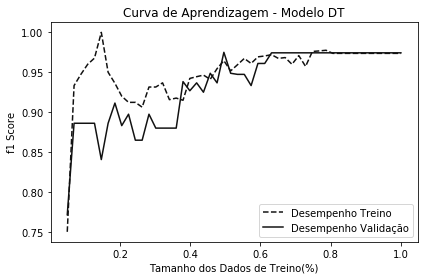
\includegraphics[width=.5\textwidth]{imagens/ca_ad.png}
      \caption{Curva de Aprendizagem do modelo de Árvore de Decisão}
      \label{fig:feature1}
    \end{figure}

    Com este mesmo gráfico é possível notar que o modelo proposto não
    foi afetado com \textit{overfitting} ou \textit{underfitting}
    \cite{HAYKIN:2001,zhang2019overfitting}. Ademais, destaca-se que o
    desempenho do modelo nos dados de validação é satisfatório. Esse
    comportamento aponta que o modelo está se ajustando corretamente
    aos dados. A mesmas percepção foi atingida nos experimentos dos
    outros modelos analisados.

    \subsection{Modelo e Análise dos dados}

    Ao submeter a base de dados ao algoritmo de Árvore de Decisão na
    intenção de prever a variável \emph{Class/ASD}, obtém-se a
    descrição do modelo de dados como definido na
    Figura~\ref{fig:model}. O modelo ilustrado relaciona a
    classificação obtida pela variável \emph{result} distribuída pela
    frequência de casos. Essa relação vem a indicar que os indivíduos
    que atendem a 7 (sete) ou mais características esperadas da TEA
    necessariamente foram clinicamente diagnosticados com o
    transtorno.\\

    \begin{figure*}[H]
      \centering
      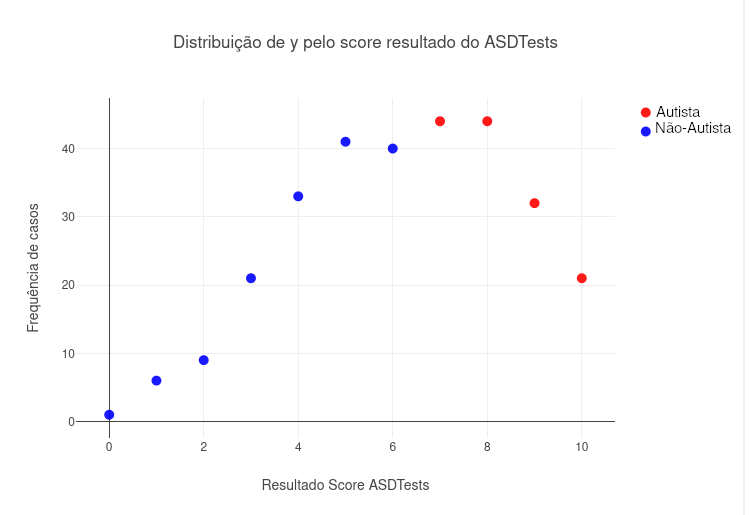
\includegraphics[width=.8\textwidth]{imagens/model.png}
      \caption{Modelo de análise dos dados}
      \label{fig:model}
    \end{figure*}


    \subsection{Avaliação da Performance do Modelo}

    Para evitar que o modelo crie um viés às condições iniciais de
    implementação, utilizou-se uma validação cruzada do tipo
    \textit{k-fold} com \emph{k = 5}. Além deste tratamento, é
    necessário avaliar a quantidade de falso-positivos e
    falso-negativos em uma amostra não observada no treinamento do
    modelo. Para tal utilizou-se a Matriz de Confusão e levou-se em
    consideração uma amostragem de 20\% dos indivíduos separados para
    teste do modelo. Dessa maneira, repetiram-se os experimentos
    \emph{k} vezes de forma com que toda a população possa ser
    testada. Os valores alcançados estão na Tabela \ref{tab:confusao2}
    e a média de falso-positivos foi de 7,692\% enquanto a média de
    falso-negativos obtida foi de 3,704\%.

    \begin{table}
      \caption{Matriz de Confusão}\label{tab:confusao2}
      \centering
      \begin{tabular}{cccc}
        &                                  & \multicolumn{2}{c}{Rótulo Previsto}                             \\ \cline{3-4}
        & \multicolumn{1}{c|}{}            & \multicolumn{1}{c|}{Autismo}
        & \multicolumn{1}{c|}{Não-Autismo} \\ \cline{2-4} \multicolumn{1}{c|}{\multirow{2}{*}{\begin{tabular}[c]{@{}c@{}}Rótulo\\ Real\end{tabular}}}
        & \multicolumn{1}{c|}{Autismo}     & \multicolumn{1}{c|}{26}
        & \multicolumn{1}{c|}{1}           \\ \cline{2-4} \multicolumn{1}{c|}{}
        & \multicolumn{1}{c|}{Não-Autismo} & \multicolumn{1}{c|}{2}       & \multicolumn{1}{c|}{27}          \\ \cline{2-4}
      \end{tabular}
    \end{table}

    \section{Conclusão}

    Os algoritmos utilizados atingiram um bom resultado nesse
    problema, chegando a superar valores de 95\% na medida F1 Score
    relacionada ao desempenho dos modelos. Os resultados obtidos foram
    influenciados por basicamente as mesmas variáveis. Assim reforça
    que mesmo com a natureza distinta dos algoritmos, houve uma mesma
    tendência de comportamento dos classificadores.

    Portanto, a metodologia proposta torna possível medir que as
    variáveis mais discriminantes e que apontam ao diagnóstico de TEA
    consistem em: facilidade de fazer múltiplas tarefas
    simultaneamente (A4), na dificuldade de fazer novas amizades (A10)
    e na percepção de baixos ruídos (A1), sendo relacionadas pela
    ausência e presença destes traços comportamentais,
    respectivamente. Ainda é possível concluir que o indivíduo que
    apresenta correspondência em sete ou mais dos dez traços
    comportamentais propostos pelo questionário possui fortes indícios
    de possuir o transtorno em algum espectro do autismo.

    Futuramente este trabalho se propõe a aplicar modelos mais
    robustos na bases de dados, como algoritmos com otimização de
    gradiente e Redes Neurais Artificiais Profundas. Além disso,
    pretende-se construir e coletar de uma base de dados junto a
    especialistas para analisar e desenvolver novos modelos
    computacionais com maior eficiência neste auxílio ao diagnóstico
    de TEA.

    \bibliographystyle{abbrv}
    \bibliography{bibtex}

  \end{document}
